% !Mode\dots ``TeX:UTF-8''
% !TEX root = ../bare_jrnl.tex

\section{Preliminaries} 
\label{sec:pre}
We now introduce the formal definition of {\BCNs} and  the control-theoretical problems  of controllability, observability and  identification. Throughout the paper, we use $\mathbb{B}$ to denote the set of Boolean values $\{0,1\}$ and $\mathbb{T}$ to denote the set of discrete time domain  $\{0,1,2, \ldots\}$ which is the set of natural numbers.

\subsection{Boolean Control Networks}

We take the definition in ~\cite{Ideker2001A} in which a Boolean control network (BN)  is given a directed graph together with two  logical equations which define the updating rules for the  values of the nodes. 

\begin{definition}[Boolean Control Network] A \BCN\ is a structure $\BB = (I,S,O, E, \sigma, \rho)$. The first four components $(I,S,O, E)$ form a directed graph which consists of 
	\begin{itemize}
	\item three nonempty disjoint sets  of nodes 
	\begin{itemize}
	\item {\bf input nodes} $I=\{\mathsf{i}_1$,\ldots ,$\mathsf{i}_{\ell}\}$
	\item {\bf state nodes}  $S= \{\mathsf{s}_1$,\ldots ,$\mathsf{s}_m\}$, and 
	\item {\bf output nodes}: $O= \{\mathsf{o}_1$,\ldots ,$\mathsf{o}_n\}$.
	\end{itemize}	
\item a set of edges 
		\[E  \subseteq ((I\cup S)\times S)\cup (S\times O)\]
\end{itemize}	
Each node at any time takes a Boolean value in $\mathbb{B}$, and $\sigma$ and $\rho$ are Boolean valued functions which define relations among the values of the nodes such that for any time $t\in  \mathbb{T}$
\begin{equation}
\begin{split}
\mathsf{s}(t+1)=&\sigma(\mathsf{i}(t),\mathsf{s}(t))\\
\mathsf{o}(t)=&\rho(\mathsf{s}(t))
\end{split}
\label{equ:1}
\end{equation}
These two functions are called the  {\bf updating rules}  of $\BB$.
 \end{definition}
It is noted that there are two sets of edges in $E$, that is $(I\cup S)\times S$ and $S\times O$. An edge $(v,v')$ represents that the value of node $v'$ is directly affected by the value of $v$, and the updating rules reflect how a node is affected by the other nodes. 

Furthermore, we use $i$ to represent a vector $(i_1,\ldots i_\ell)$ of input values, $s$ a vector $(s_1,\ldots s_m)$ of state values, and $o$ a vector $(o_1,\ldots o_n)$ of output values, which called an {\em input}, a {\em state} and an {\em output} for simplicity.  And at any time $t\in \mathbb{T}$ during the execution of $\BB$, we use $i(t)$, $s(t)$, and $o(t)$ to represent the input $(i_1(t),\ldots i_\ell(t))$, state $(s_1(t),\ldots s_m(t))$  and  output $(o_1(t),\ldots o_n(t))$ at time $t$, respectively. We use $\mathcal{I}_\BB$, and $\mathcal{S}_\BB$ and $\mathcal{O}_\BB$ to represent the sets of all possible inputs, states and outputs of $\BB$, respectively. And we will omit the subscript $\BB$ when there is no confusion. Obviously, $\mathcal{I}_\BB$, and $\mathcal{S}_\BB$ and $\mathcal{O}_\BB$ are finite with $2^\ell$, $2^m$ and $2^n$ elements, respectively.


\begin{figure}[!t]
      \centering
      \framebox{\parbox{3in}{
		\centerline{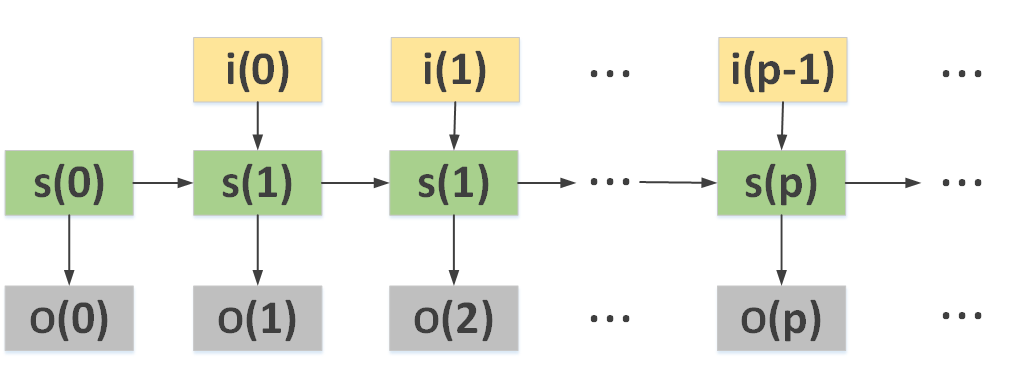
\includegraphics[scale=0.17]{figures/Fig10.png}}
	}}
      
      \caption{The relationship of inputs, states and outputs.}
      \label{fig:10}
  \end{figure}
%===========================================================
\begin{example}\label{exa:2}
	 \begin{figure}[thpb]
		\centering
		\framebox{\parbox{3in}{
				\centerline{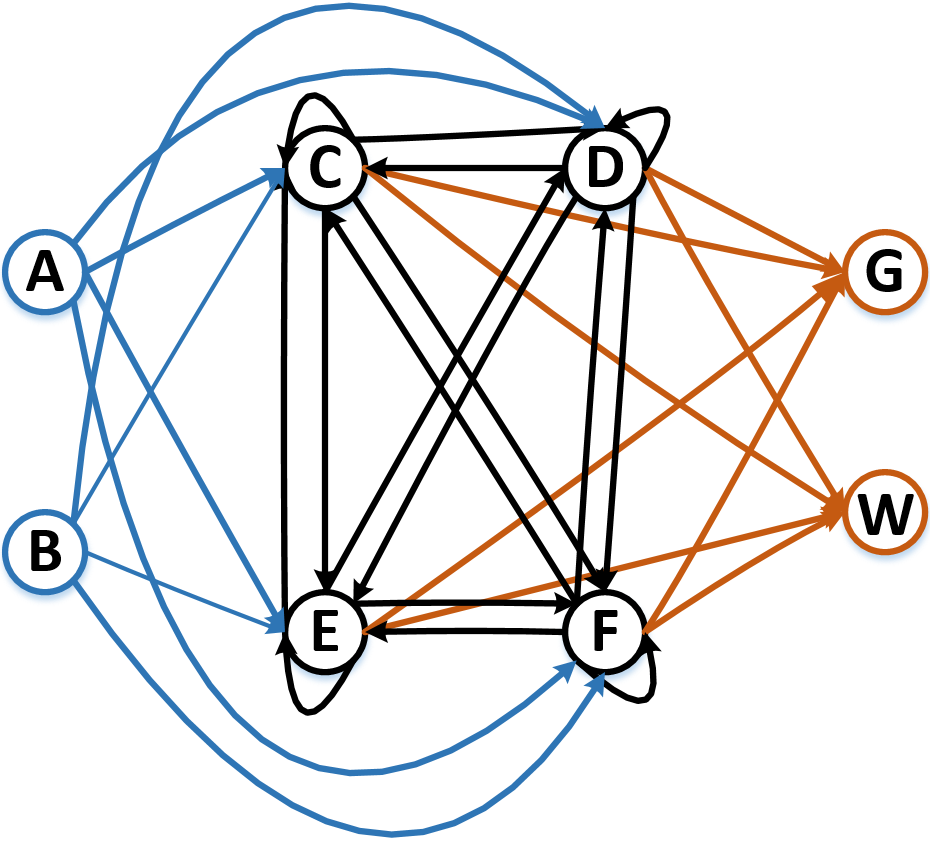
\includegraphics[scale=0.23]{figures/Fig1.png}}
		}}
		
		\caption{A Boolean control network. }%We use blue, black and orange, to distinguish three types of nodes and three types of edges. with two input-nodes $A$ and $B$, four state-nodes $C$, $D$, $E$ and $F$, and two output-nodes $G$, $W$.
		\label{fig:1}
	\end{figure}
%	
Let $\BB$ be the \BCN\  shown in Fig.~\ref{fig:1} which has two  input-nodes $I=\{i_1,i_2\}$ , four state-nodes $S=\{s_1, s_2,s_3, s_4\}$ and two output-nodes $O=\{o_1,o_2\}$. 
The updating rules $\sigma: \mathbb{B}^{6}\mapsto \mathbb{B}^4$ and $\rho:\mathbb{B}^4\mapsto \mathbb{B}^2$ are given in the truth table (Fig.~\ref{fig:2}) from which the updating rules in terms of logic functions can be easily recovered.   For instance, %from the truth table we have 
the updating rule of output-node $o_1$ is 
$o_1(t)=s_1(t)\vee {({s_2}(t)\wedge { s_3}(t)\wedge {s_4}(t))}.$
 \begin{figure}[thpb]
	\centering
	\framebox{\parbox{3in}{
			\centerline{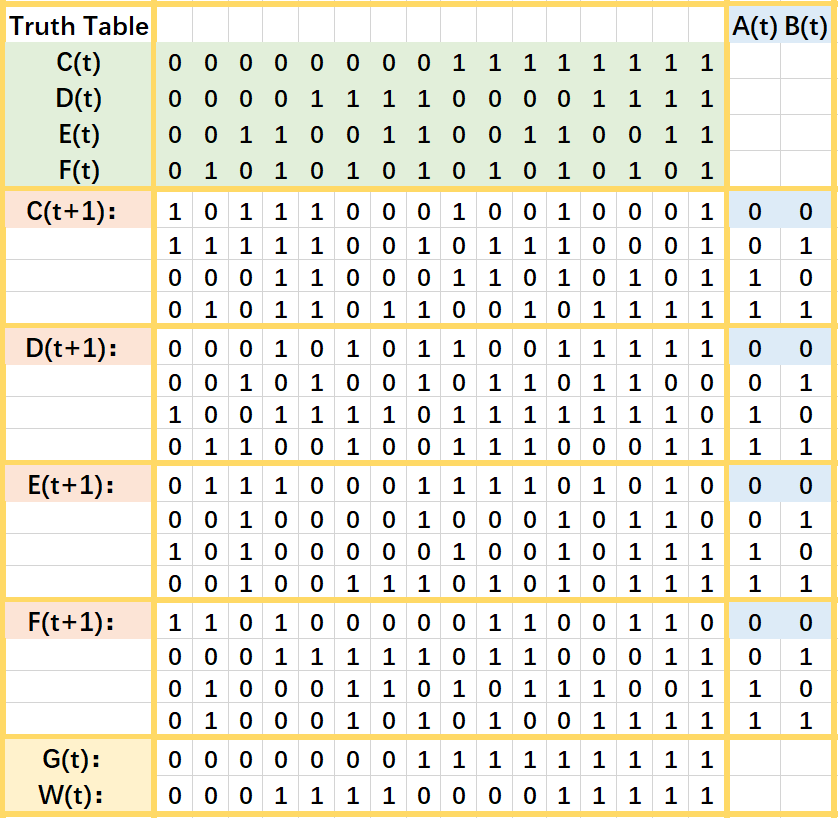
\includegraphics[scale=0.261]{figures/Fig2.png}}
	}}
	\caption{The truth table which describe the updating rules of the \BCN\ shown in Fig.~\ref{fig:1}.}
	\label{fig:2}
\end{figure}
%For instance, from the truth table we have the updating rule of output-node $G$ is 
%$G(t)=C(t)\vee {({D}(t)\wedge { E}(t)\wedge {F}(t))}.$
 %
\end{example}   

%===========================================================

%The reason why we use the truth table to describe the updating rules of the \BCN\ is that it would be more convenient for us to convert the $\mathsf{i}(t)$, $\mathsf{s}(t)$ and $\mathsf{o}(t)$ into their abbreviation forms. 
%That we use 
%\begin{itemize}
%  \item $\delta^i_{2^m}$ represents the abbreviation form of $\mathsf{i}(t)$, where $i=\sum_{x=1}^m \mathsf{i}_{x}(t)\times 2^{m-x}$;
%  \item $\delta^j_{2^n}$ represents the abbreviation form of $\mathsf{s}(t)$, where $j=\sum_{x=1}^n \mathsf{s}_{x}(t)\times 2^{n-x}$;
%  \item $\delta^w_{2^q}$ represents the abbreviation form of $\mathsf{o}(t)$, where  $w=\sum_{x=1}^q \mathsf{o}_{x}(t)\times 2^{q-x}$.
%\end{itemize}
%
%For instance if $\mathsf{s}(t)=\begin{bmatrix}\mathsf{s}_1(t)\\\mathsf{s}_2(t) \\ \mathsf{s}_3(t) \\\mathsf{s}_4(t)\end{bmatrix}=\begin{bmatrix}0\\1\\0\\1\end{bmatrix}$, then $\mathsf{s}(t)$ can be represented by $\delta^{(0\times2^3+1\times2^2+0\times2^1+1\times2^0)}_{2^4}=\delta^5_{16}$. 
%
%In the \BCN\ which shown in the Fig.~\ref{fig:1}, we consider 
%\begin{itemize}
%  \item $A(t)$ as $\mathsf{i}_{1}(t)$, $B(t)$ as $\mathsf{i}_{2}(t)$;
%  \item $C(t)$ as $\mathsf{s}_{1}(t)$, $D(t)$ as $\mathsf{s}_{2}(t)$;
%  \item $E(t)$ as $\mathsf{s}_{3}(t)$, $F(t)$ as $\mathsf{s}_{4}(t)$;
%  \item $G(t)$ as $\mathsf{o}_{1}(t)$, $W(t)$ as $\mathsf{o}_{2}(t)$.
%\end{itemize}
%
%Then, the updating rules which shown in Fig.~\ref{fig:2} can be represented by Fig.~\ref{fig:6}.
% \begin{figure}[thpb]
%      \centering
%      \framebox{\parbox{3in}{
%		\centerline{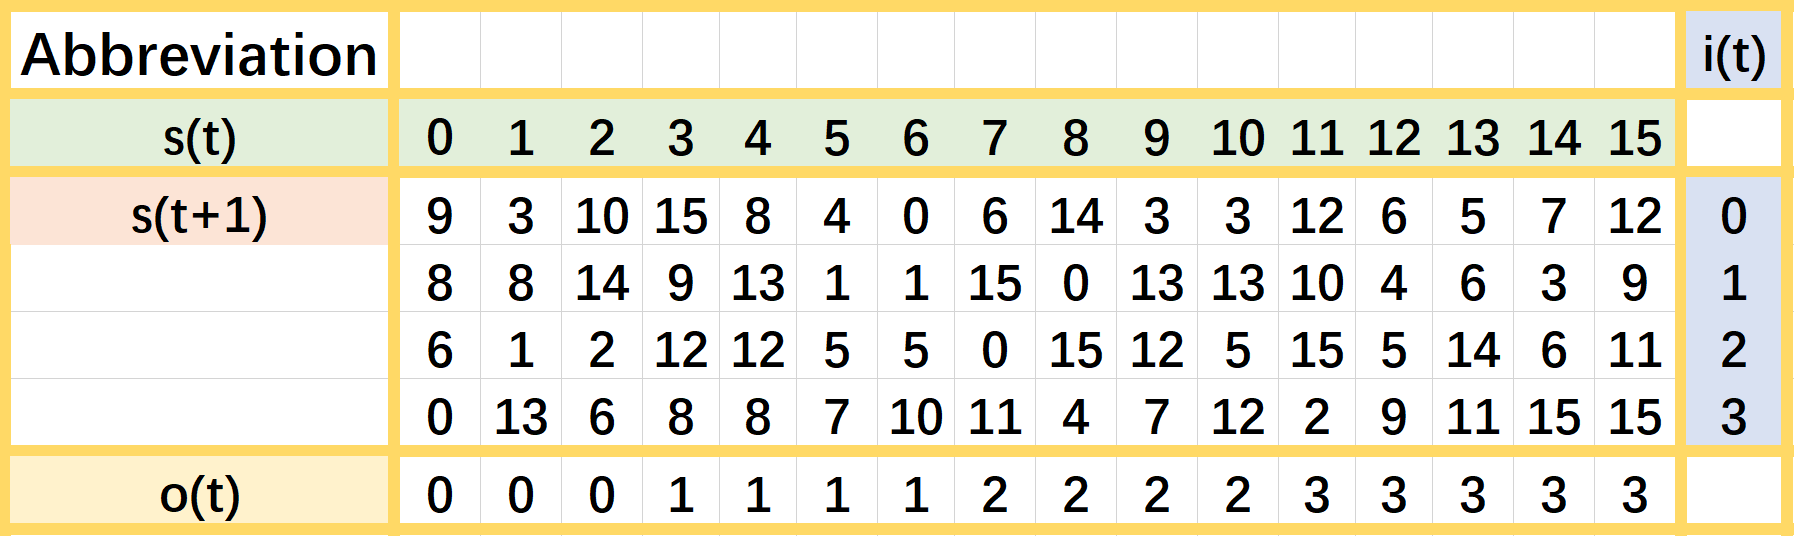
\includegraphics[scale=0.122]{figures/Fig7.png}}
%	}}
%      
%      \caption{The abbreviation form of the updating rules.}
%      \label{fig:6}
%   \end{figure}
%  
%   With the abbreviation forms of $\mathsf{i}(t)$, $\mathsf{s}(t)$ and $\mathsf{o}(t)$, it would be easier for us to use this \BCN\ to explain various concepts by checking this table.
  % 
%For instance, if $\mathsf{s}(t)=\delta^5_{16}$ and $\mathsf{i}(t)=\delta^1_{4}$, then we can know that $\mathsf{s}(t+1)=\delta^4_{16}$  and $\mathsf{s}(t+1)=\delta^1_{4}$ by checking this table.   
 % \tl{(1)simplify later?!} 
%   \begin{itemize}
% \item $\Delta_M = \{\delta^0_{2^m},\ldots,\delta^{({2^m}-1)}_{2^m} \}$ represents the input set; 
% \item $\Delta_N = \{\delta^0_{2^n},\ldots,\delta^{({2^n}-1)}_{2^n} \}$ represents the state set; 
% \item $\Delta_Q = \{\delta^0_{2^q},\ldots,\delta^{({2^q}-1)}_{2^q} \}$ represents the output set,
%\end{itemize}
%where $M=2^m$, $N=2^n$ and $Q=2^q$.
%=======================================================================

%=======================================================================


\subsection{Four existing observability definitions of \BCNs}
To introduce the observability, controllability and identifiability of \BCNs, we first define the mappings \cite{Zhang2016Observability}:
\begin{equation}
\begin{split}
F^k_{\mathsf{s}(t)}:& (\Delta_L)^k\mapsto(\Delta_M)^k\\
&=\mathsf{i}(t)\ldots\mathsf{i}({t+k-1}) \mapsto \mathsf{s}(t+1)\ldots\mathsf{s}(t+k)\\
(HF)^k_{\mathsf{s}(t)} :& (\Delta_L)^k\mapsto(\Delta_N)^k\\
 &=\mathsf{i}(t)\ldots\mathsf{i}(t+k-1) \mapsto \mathsf{o}(t+1)\ldots\mathsf{o}(t+k)
\end{split}
\label{equ:6}
\end{equation}
%\tl{but you have defined $\Delta_N$, $\Delta_M$ and $\Delta_Q$ just now?!}
where $k>0$. For all  $k>0$,
$\mathsf{I}[k]=\mathsf{i}(t)\ldots\mathsf{i}({t+k-1}) \in(\Delta_L)^k$
is an input sequence, 
$F^k_{\mathsf{s}(t)}(\mathsf{I}[k])=\mathsf{s}(t+1)\ldots\mathsf{s}(t+k) \in(\Delta_M)^k$
 is a state sequence, and 
 $(HF)^k_{\mathsf{s}(t)}(\mathsf{I}[k])=\mathsf{o}(t+1)\ldots\mathsf{o}(t+k) \in(\Delta_N)^k$
 is an output sequence. That for every $1\le x \le k$, 
 $\mathsf{s}(t+x)=\sigma(\mathsf{i}(t+x-1),\mathsf{s}(t+x-1))$,
and 
 $\mathsf{o}(t+x)=\rho(\mathsf{s}(t+x))=\rho(\sigma(\mathsf{i}(t+x-1),\mathsf{s}(t+x-1)))$.



Then, the observability, controllability and identifiability of \BCNs\ are defined as follows.

\begin{definition} [{\bf Type-I} Observability~\cite{cheng2009controllability}]
The {\bf Type-I} observability is that, a \BCN\ is observable if for every initial state \State$(0)\in \Delta_M$, there exists an input sequence $\mathsf{I}[k]\in(\Delta_L)^k$ for some $k>0$, such that for all states $\mathsf{s}'(0)\neq \mathsf{s}(0)$, $\rho(\mathsf{s}'(0))=\rho(\mathsf{s}(0))$ implies $(HF)^k_{\mathsf{s}'(0)}(\mathsf{I}[k])\neq (HF)^k_{{\mathsf{s}(0)}}(\mathsf{I}[k])$.
\end{definition}

The  {\bf Type-I} observability means that a \BCN\ is observable if every \State$(0)$ of the \BCN\ can be distinguished from other types of initial state by an input sequence $\mathsf{I}[k]$. %Thus, we can only check whether $\mathsf{s}(0)=\mathsf{s}^{x}(0)$ or not by $\mathsf{I}^x$. %
\begin{example}
For example, for the \BCN\ mentioned in {\em Example \ref{exa:2}}, we have every \State$(0)$ can be distinguished from other types of initial state by an $\mathsf{I}[k] \in(\Delta_L)^k$.  For instance,
\begin{itemize}
  \item $\delta_{16}^0$ can be distinguished from other types of initial state by any $\mathsf{I}[k]$ with the prefix $\delta_{4}^3$, $\delta_{4}^2$ or $\delta_{4}^0  \delta_{4}^2$;%
  \item $\delta_{16}^1$ can be distinguished from other types of initial state by any $\mathsf{I}[k]$ with the prefix $\delta_{4}^0$, $\delta_{4}^3$ or $\delta_{4}^2 \delta_{4}^3$;
  \item $\delta_{16}^2$ can be distinguished from other types of initial state by any $\mathsf{I}[k]$ with the prefix $\delta_{4}^1$, $\delta_{4}^3$ or $\delta_{4}^0 \delta_{4}^2$, etc.
\end{itemize} 
Therefore, this \BCN\ satisfies the  {\bf Type-I} observability.
\label{exa:4}
\end{example}   

\begin{definition}[ {\bf Type-II} Observability~\cite{Zhao2010Input}]
	The  {\bf Type-II} observability is that, a \BCN\ is observable if for every two distinct initial states $\mathsf{s}(0)$, $\mathsf{s}'(0) \in \Delta_M$, there is an input sequence $\mathsf{I}[k]\in(\Delta_L)^k$ for some $k>0$, such that $\rho(\mathsf{s}(0))=\rho(\mathsf{s}'(0))$ implies $(HF)^k_{\mathsf{s}(0)}(\mathsf{I}[k])\neq (HF)^k_{\mathsf{s}'(0)}(\mathsf{I}[k])$.
\end{definition}

The {\bf Type-II} observability means that a \BCN\ is observable if for every two distinct $\mathsf{s}(0)$, $\mathsf{s}'(0)$, there is an input sequence $\mathsf{I}[k]$ which distinguishes them. %Therfore, we can only check $\mathsf{s}(0)=\mathsf{s}^{x}(0)$ or $\mathsf{s}(0)=\mathsf{s}^{y}(0)$ when we know that $\mathsf{s}(0)$ is one of them by $\mathsf{I}^{xy}$. 
\begin{example}
For example, for the \BCN\ mentioned in {\em Example \ref{exa:2}}, we have for every two distinct $\mathsf{s}(0)$ and $\mathsf{s}'(0)$, there exists an $\mathsf{I}[k]\in(\Delta_L)^k$ which can distinguish them.  For instance,
\begin{itemize}
  \item $\mathsf{I}[k]$ with the prefix $\delta_{4}^0$ can distinguish $\delta_{16}^0$ and $\delta_{16}^1$;
  \item $\mathsf{I}[k]$ with the prefix $\delta_{4}^1$ can distinguish $\delta_{16}^0$ and $\delta_{16}^2$;
  \item $\mathsf{I}[k]$ with the prefix $\delta_{4}^3$ can distinguish $\delta_{16}^1$ and $\delta_{16}^2$.
\end{itemize} 
Therefore this \BCN\ satisfies the {\bf Type-II} observability.
\label{exa:5}
\end{example}   
\begin{definition}[{\bf Type-III} Observability~\cite{Cheng2011Identification}]
The {\bf Type-III} observability is that, a \BCN\ is observable if there exists an input sequence $\mathsf{I}[k]\in(\Delta_L)^k$ for some $k>0$, such that for any two distinct states $\mathsf{s}(0)$, $\mathsf{s}'(0) \in \Delta_M$, $\rho(\mathsf{s}(0))=\rho(\mathsf{s}'(0))$ implies $(HF)^k_{\mathsf{s}(0)}(\mathsf{I}[k])\neq (HF)^k_{\mathsf{s}'(0)}(\mathsf{I}[k])$.
\end{definition}

The {\bf Type-III} observability means that a \BCN\ is called observable if there exists an input sequence $\mathsf{I}[k]$ which determine the $\mathsf{s}(0)$ of the \BCN\ for every $\mathsf{s}(0)\in\Delta_M$, because $\mathsf{I}[k]$ can distinguish all distinct initial states.%, the $\mathsf{s}(0)$ is determined by its corresponding output sequence $(HF)^k_{\mathsf{s}(0)}(\mathsf{I})$.

\begin{example}
For example, for the \BCN\ mentioned in {\em Example \ref{exa:2}}, for any $k>0$, there is not an $\mathsf{I}[k]\in(\Delta_L)^k$ which determines the $\mathsf{s}(0)$ of this \BCN:
\begin{itemize}
  \item $\mathsf{I}[k]$ with prefix $\delta_{4}^0$ can not distinguish $\delta_{16}^9$ and $\delta_{16}^{10}$;
  \item $\mathsf{I}[k]$ with prefix $\delta_{4}^1$ can not distinguish $\delta_{16}^0$ and $\delta_{16}^{1}$;
  \item $\mathsf{I}[k]$ with prefix $\delta_{4}^2$ can not distinguish $\delta_{16}^3$ and $\delta_{16}^{4}$;
  \item $\mathsf{I}[k]$ with prefix $\delta_{4}^3$ can not distinguish $\delta_{16}^{14}$ and $\delta_{16}^{15}$.
\end{itemize} 
Therefore it does not satisfy the {\bf Type-III} observability. 
\label{exa:6}
\end{example}  
\begin{definition}[{\bf Type-IV} Observability~\cite{Fornasini2013Observability}]
	The {\bf Type-IV} observability is that, a \BCN\ is observable, if there is a  natural number $N$, such that for every input sequence $\mathsf{I}[k]\in(\Delta_L)^{k}$, for any two distinct states $\mathsf{s}(0)$, $\mathsf{s}'(0) \in \Delta_M$, $\rho(\mathsf{s}(0))=\rho(\mathsf{s}'(0))$ implies $(HF)^{k}_{\mathsf{s}(0)}(\mathsf{I}[k])\neq (HF)^{k}_{\mathsf{s}'(0)}(\mathsf{I}[k])$ if  $k\ge N$.
\end{definition}

The {\bf Type-IV} observability means that a \BCN\ is observable if every sufficient long $\mathsf{I}[k]$ can determine the $\mathsf{s}(0)$ of the \BCN\ for every $\mathsf{s}(0)\in\Delta_N$.%, because every sufficient long $\mathsf{I}[k]$ can distinguish any two distinct initial states.%, the $\mathsf{I}$ can be determined by its output sequence $(HF)^k_{\mathsf{s}(0)}(\mathsf{I})$.
\begin{example}
For example, for the \BCN\ mentioned in {\em Example \ref{exa:2}}, any $\mathsf{I}[k]$ with prefix $\delta_{4}^0$ can not can not distinguish $\delta_{16}^9$ and $\delta_{16}^{10}$. 
Therefore this \BCN\ does not satisfy the {\bf Type-IV} observability. 
\label{exa:7}
\end{example}  

The implication relationships of four existing types of observability shown in Fig.~\ref{fig:9}. For the details of its proving process, we refer readers to \cite{Zhang2016Observability}.

 \begin{figure}[thpb]
     \centering
    \framebox{\parbox{3in}{
		\centerline{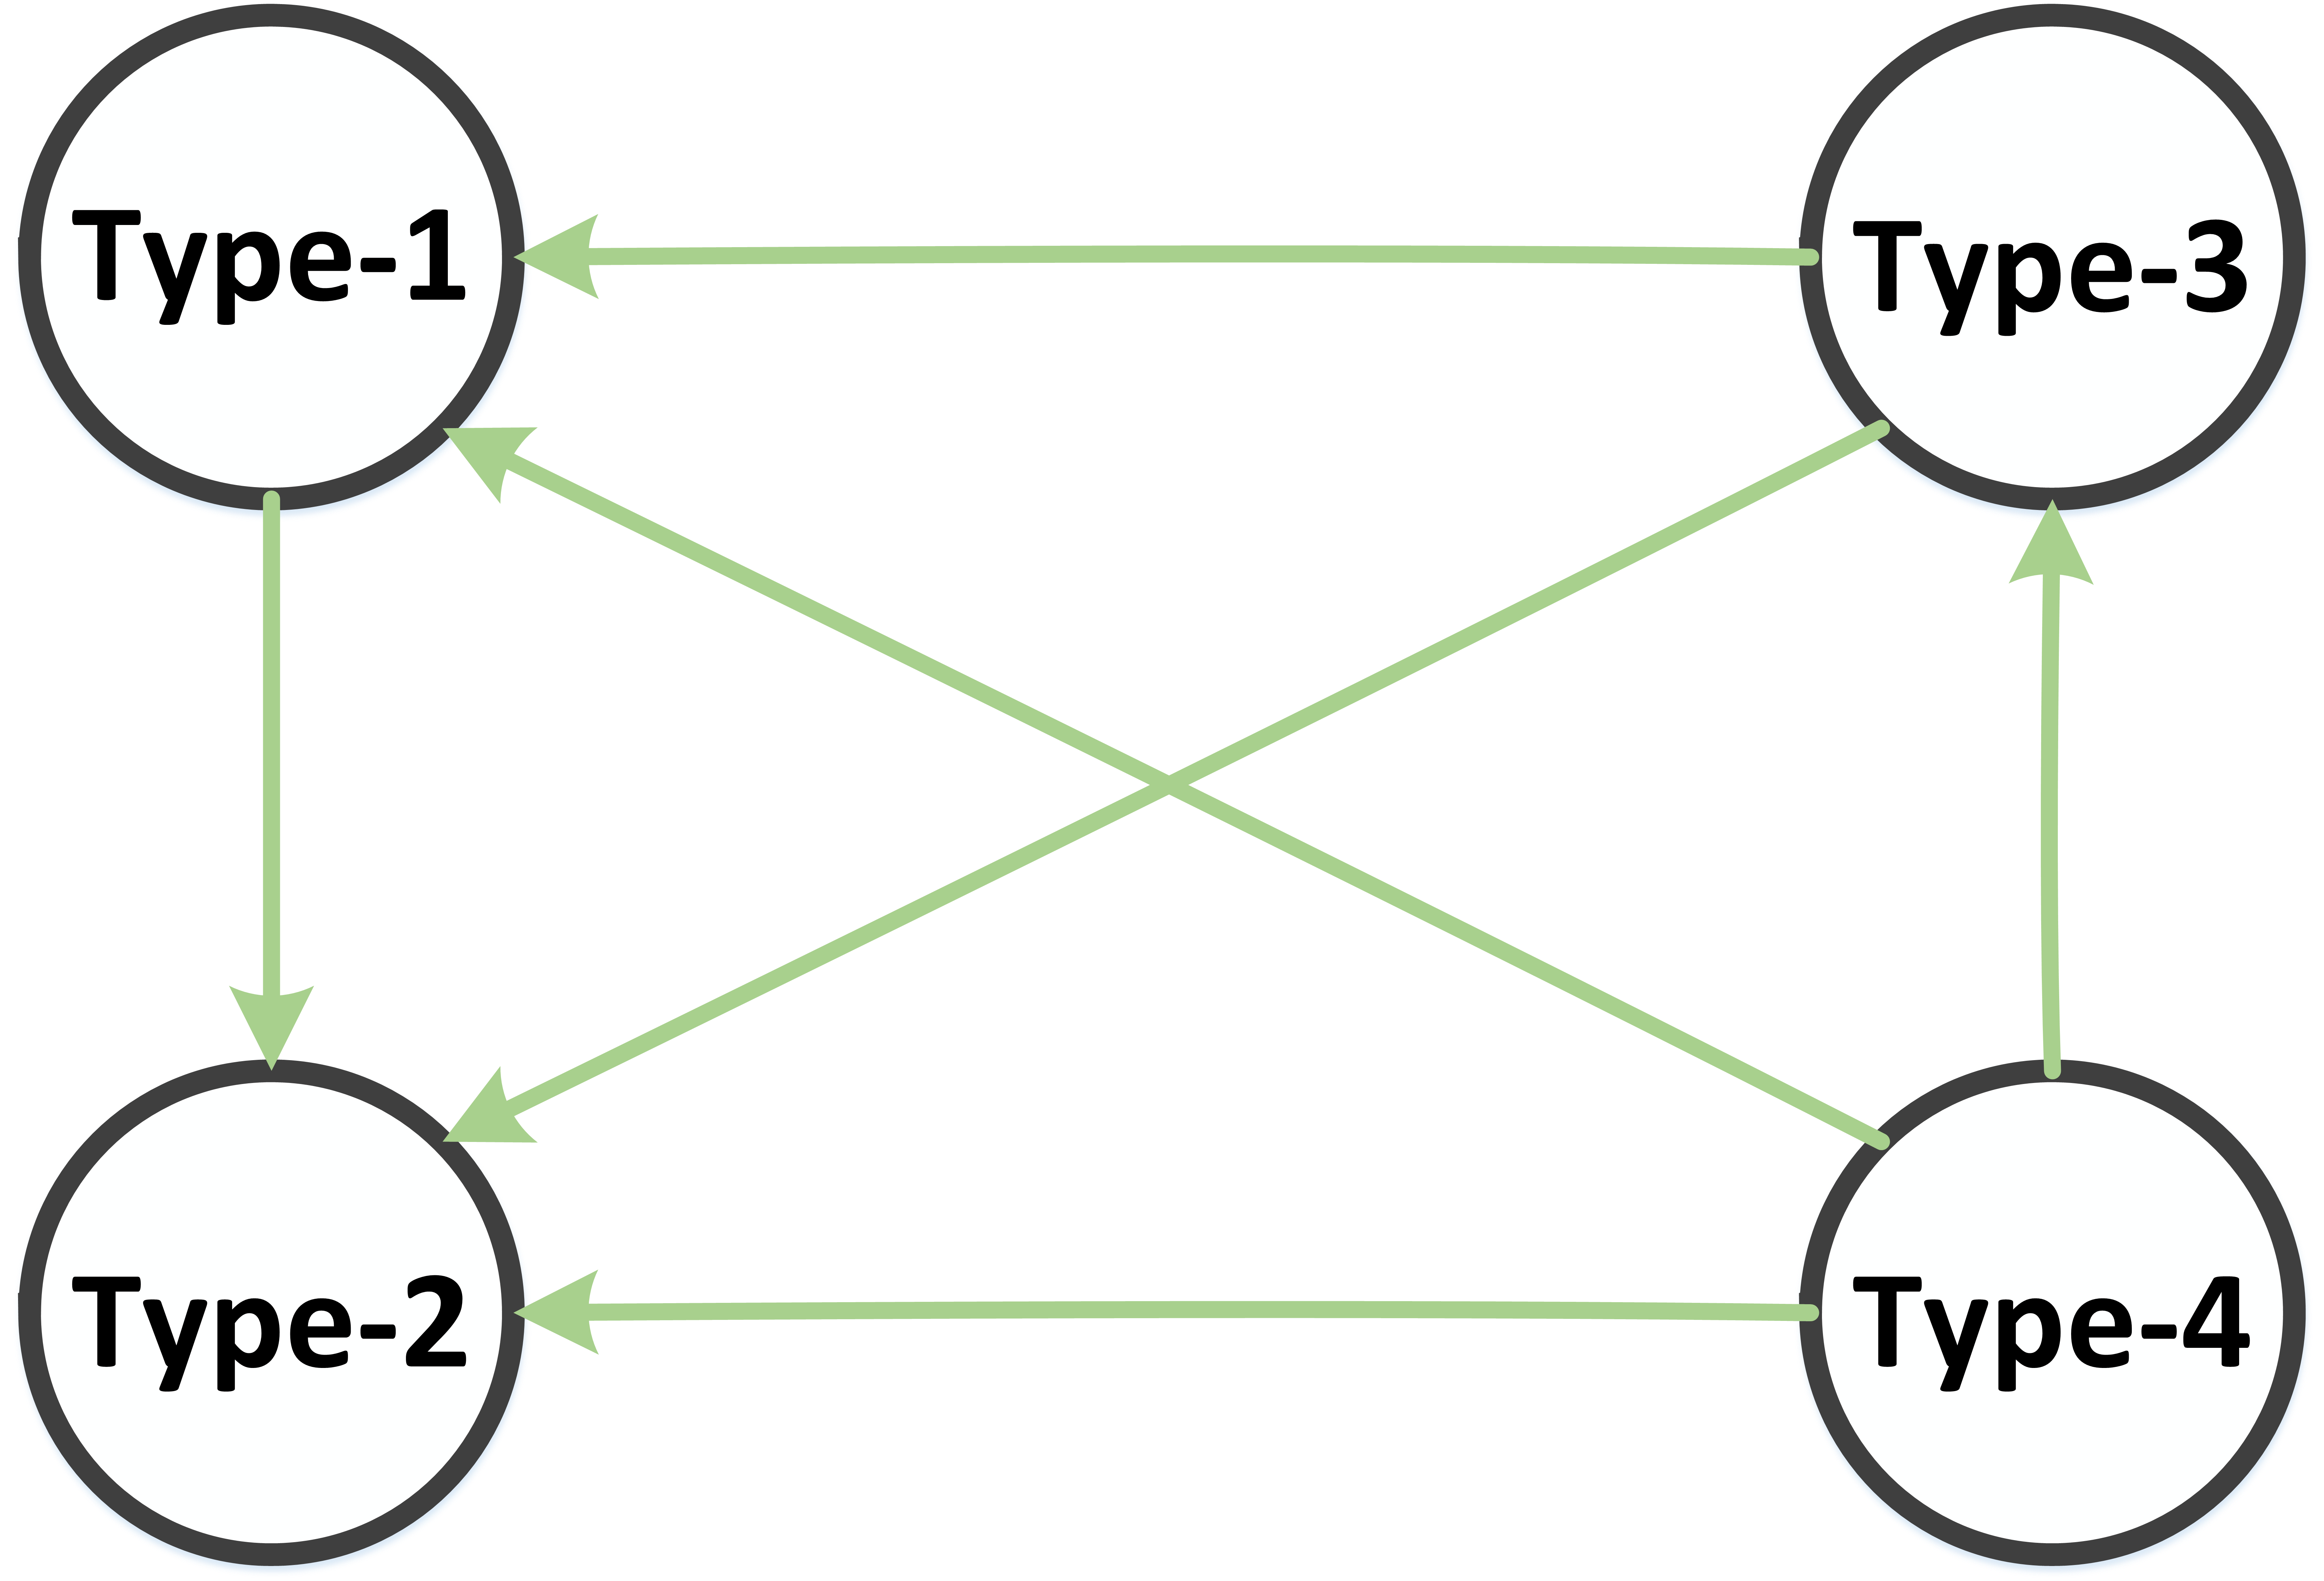
\includegraphics[scale=0.27]{figures/Fig9.png}}
	}}
      
     \caption{The implication relationships graph between observability {\bf Type-I}, {\bf Type-II}, {\bf Type-III} and {\bf Type-IV}, where ``$\rightarrow$" means ``implies".}
      \label{fig:9}
   \end{figure}

%The implication relationship is that ``The first observability implies the second observability.'' means ``If a \BCN\ satisfies the first observability, then it satisfies the second observability.'' 



%\subsection{Controllability and identifiability of \BCNs}
%\tl{what's the point here?}


\begin{definition}[Controllability~\cite{cheng2009controllability}]
	A \BCN\ is controllable if for any initial state $\mathsf{s}(0)$ and destination state $\mathsf{s}'$, there is an input sequence $\mathsf{I}[k]\in(\Delta_L)^k$ for some $k>0$, such that in $F^k_{\mathsf{s}(0)}(\mathsf{I}[k])=\mathsf{s}(1) \ldots\, \mathsf{s}(k)$, the $\mathsf{s}(k)=\mathsf{s}'$.
\end{definition}

\begin{example}
For example, the \BCN\ mentioned in {\em Example \ref{exa:2}} is controllable, that is for any initial state $\mathsf{s}(0)$ and destination state $\mathsf{s}'$, there is an input sequence $\mathsf{I}[k]$, such that in the $F^k_{\mathsf{s}(0)}(\mathsf{I}[k])=\mathsf{s}(1) \ldots\, \mathsf{s}(k)$, the $\mathsf{s}(k)=\mathsf{s}'$. For instance, for the initial state $\mathsf{s}(0)= \delta_{16}^{1}$ and destination state $\mathsf{s}'=\delta_{16}^{2}$, there is an input sequence $\mathsf{I}[3]=\delta_{4}^{3}\delta_{4}^{3}\delta_{4}^{3}$, such that $F^3_{\delta_{16}^{1}}(\delta_{4}^{3}\delta_{4}^{3}\delta_{4}^{3})=\delta_{16}^{13}\delta_{16}^{11}\delta_{16}^{2}$.
\label{exa:12}
\end{example}  

\begin{definition}[Identifiability~\cite{Cheng2011Identification}]%
	A \BCN\ is identifiable if there exists an input sequence $\mathsf{I}[k]\in(\Delta_L)^k$ for some $k>0$, such that the updating rules
	\begin{equation*}
    		\begin{split}
		\mathsf{s}(t+1)=&\sigma(\mathsf{i}(t),\mathsf{s}(t))\\
		\mathsf{o}(t)=&\rho(\mathsf{s}(t))
		\end{split}
	\end{equation*}
	can be determined by $\mathsf{I}[k]$ and $(HF)^k_{\mathsf{s}(0)}(\mathsf{I}[k])$.
\end{definition}

%\begin{definition}[Observability]
%A \BCN\ $\BB$ is observable if there exists an input sequence $\mathsf{I}\in(\Delta_L)^k$ for some $k>0$, such that for any two distinct states $\mathsf{s}(0)$, $\mathsf{s}'(0) \in \Delta_M$, $h(\mathsf{s}(0))=h(\mathsf{s}'(0))$ implies $(HF)^k_{\mathsf{s}(0)}(\mathsf{I})\neq (HF)^k_{\mathsf{s}'(0)}(\mathsf{I})$ \cite{Cheng2011Identification}.
%\end{definition}

%The observability means that a \BCN\ is called observable if there exists an input sequence $\mathsf{I}\in(\Delta_L)^k$ which determine the $\mathsf{s}(0)$ of the \BCN\ for every $\mathsf{s}(0)\in\Delta_M$, because $\mathsf{I}$ can distinguish any two distinct initial states.%, the $\mathsf{s}(0)$ is determined by its corresponding output sequence $(HF)^k_{\mathsf{s}(0)}(\mathsf{I})$.

%\begin{example}
%For example, for the \BCN\ mentioned in {\em Example \ref{exa:2}}, for any $k>0$, there is not any $\mathsf{I}\in(\Delta_L)^k$ which can determine the $\mathsf{s}(0)$ of this \BCN:
%\begin{itemize}
 % \item any $\mathsf{I}$ with prefix $\delta_{4}^0$ can not distinguish $\delta_{16}^9$ and $\delta_{16}^{10}$;
 % \item any $\mathsf{I}$ with prefix $\delta_{4}^1$ can not distinguish $\delta_{16}^0$ and $\delta_{16}^{1}$;
  %\item any $\mathsf{I}$ with prefix $\delta_{4}^2$ can not distinguish $\delta_{16}^3$ and $\delta_{16}^{4}$;
%  \item any $\mathsf{I}$ with prefix $\delta_{4}^3$ can not distinguish $\delta_{16}^{14}$ and $\delta_{16}^{15}$.
%\end{itemize} 
%Therefore it does not satisfy the observability. 
%\label{exa:6}
%\end{example}  

A \BCN\ $\BB$ is identifiable iff $\BB$ is controllable and $\BB$'s initial state $\mathsf{s}(0)$ can be determined  without  resetting~\cite{Cheng2011Identification}. And in \cite{Cheng2011Identification}, the authors regard the {\bf Type-III} observability as the necessary and sufficient condition of determining the initial state $\mathsf{s}(0)$  without  resetting. But we discover that the  {\bf Type-III} observability is sufficient but not necessary condition. Thus, we propose the online observability to present the necessary and sufficient condition.
%, because the initial state $\mathsf{s}(0)$ of a \BCN\ $\BB$ can be determined by the algorithm (mentioned in {\em Section \ref{sec:intro}}) corresponding to {\bf Type-III} observability when $\BB$ satisfies the {\bf Type-III} observability.


   
% Because we do not make full use of the output and input in the process of determining the initial state. The output of \BCNs\ we observe at every time step can help us further determine the range of the initial state. With the range of the initial state, we can use different input sequence to determine the initial state. While in the third and fourth existing observability, we use the same input sequence $\mathsf{I}$ to determine the initial state.

 
%However, in some biological systems which depicted by \BCNs, the initial states of them can be checked at most once. Therefore,
%The {\bf Type-I} observability and {\bf Type-II} observability are designed to determine the initial states of \BCNs\ when their initial state can be reset. The {\bf Type-IV} observability is designed to study the reconstructibility of \BCN. The {\bf type-III} observability is proposed to research the identification of \BCNs. In this paper, we want to use the new observability we propose to replace the {\bf Type-III} observability, such that we can research the identification problem better.
%As the first observability and second observability are designed to determine the initial states of \BCNs\ by taking the determining procedure multiple times in parallel. %\tl{why this claim?} 
%And in some applications, we have to determine \BCNs' initial states by taking the determining procedure once. The third and fourth observability are designed to determine the initial states of \BCNs\ by taking the determining procedure once. But if a \BCN\ is not satisfy the third observability, we can not use them to determine its initial states by taking the determining procedure once.  %Thus, we propose the online observability of \BCNs\ to solve the problem.
%Moreover, in some biological systems, it would takes many costs to check these biological systems. Hence it would cost a lot of overhead for us to determine the initial state of them by the first observability and second observability.





% \begin{problem}
%\label{pro:2}
%What is the necessary and sufficient condition of determining a \BCN's initial state $\mathsf{s}(0)$ by taking the determining procedure once?
%\end{problem}

